\documentclass[border=5mm]{standalone}
\usepackage{tikz}
\begin{document}
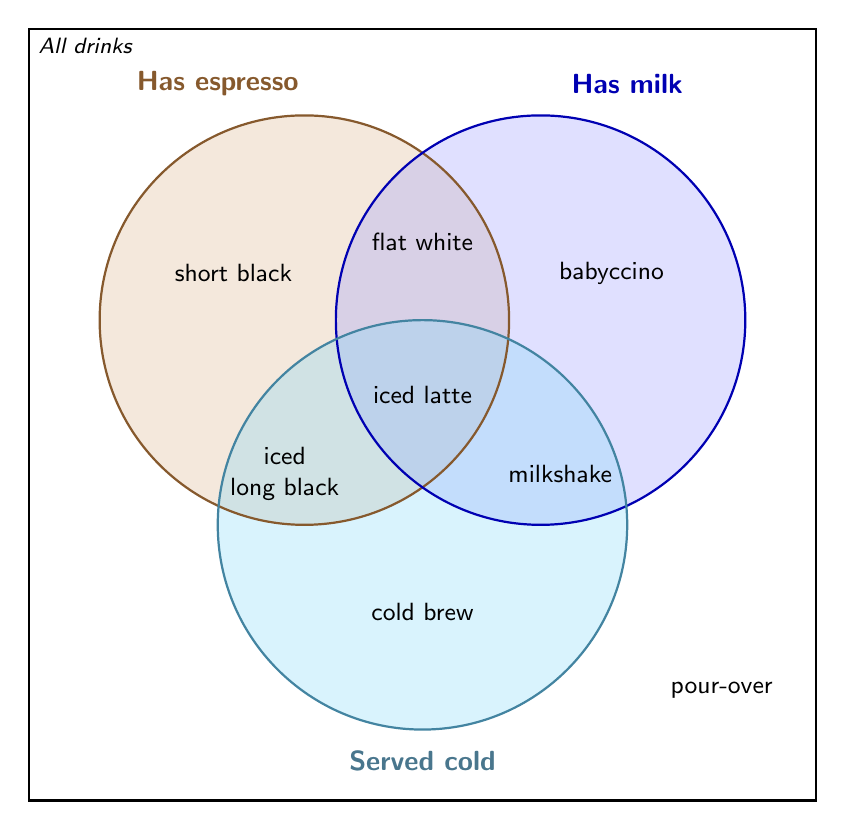
\begin{tikzpicture}[font=\sffamily\small]
\def\r{2.6}
\coordinate (E) at (-1.5,0.9);
\coordinate (M) at (1.5,0.9);
\coordinate (C) at (0,-1.7);
\draw[thick] (-5,-5.2) rectangle (5,4.6);
\node[anchor=north west,font=\sffamily\footnotesize\itshape] at (-5,4.6) {All drinks};
\fill[brown!60,opacity=.3] (E) circle (\r);
\fill[blue!40,opacity=.3] (M) circle (\r);
\fill[cyan!50,opacity=.3] (C) circle (\r);
\draw[thick,brown!70!black] (E) circle (\r);
\draw[thick,blue!70!black] (M) circle (\r);
\draw[thick,cyan!60!black] (C) circle (\r);
\node[font=\sffamily\bfseries,brown!70!black] at (-2.6,3.9) {Has espresso};
\node[font=\sffamily\bfseries,blue!70!black] at (2.6,3.9) {Has milk};
\node[font=\sffamily\bfseries,cyan!50!black] at (0,-4.7) {Served cold};
% regions
\node at (-2.4,1.5) {short black};
\node at (2.4,1.5) {babyccino};
\node at (0,-2.8) {cold brew};
\node at (0,1.9) {flat white};
\node at (0,-0.05) {iced latte};
\node[align=center] at (-1.75,-1.05) {iced\\long black};
\node at (1.75,-1.05) {milkshake};
\node at (3.8,-3.8) {pour-over};
\end{tikzpicture}
\end{document}
